\section{Parser}

In our recursive-descent Parser we implemented all EBNF (see \label{labelEBNF}) production rules as
methods. The production rules of our EBNF allows alternatives, repetitions and optional parts.
%Figure (\ref{parser_deb}) shows a dependence diagram of the parser methods.  

To ensure that our EBNF is LL(1) conform, we created the a list with first sets.
The parser compares the actual token with the first-sets symbols
and takes decisions between alternatives. 
To guarantee that the decision between two alternatives is correct, the first
set of the alternatives must be disjunctive. See apendix \ref{first_sets} for the first sets. We checked our EBNF with the Parser tool: coco, to
ensure we are are LL(1) conform. % coco page http://www.ssw.uni-linz.ac.at/Research/Projects/Coco/

%\begin{figure}[h]
%\label{parser_deb}
%\begin{center}
%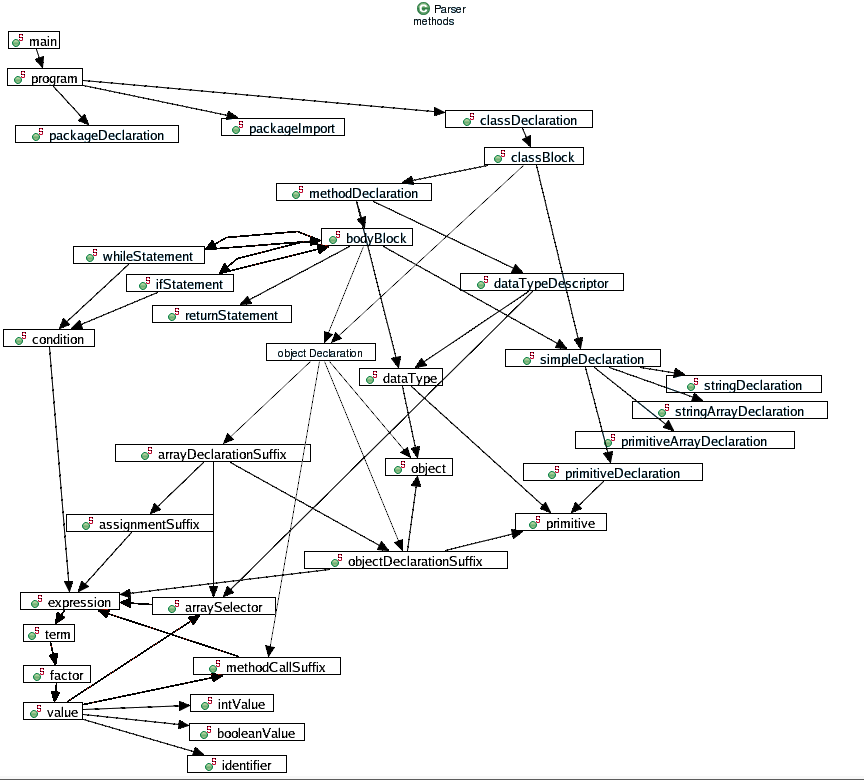
\includegraphics[width=13cm,height=13cm]{images/parser_edit.png}
%\end{center}
%\caption{parser methods dependencies}
%\end{figure}



%


\subsection{Syntax error handling}
The parser is able to detect many syntax errors. We distinguish between two error levels : weak- and strong error levels.
\begin{itemize}
  \item \textbf{Weak errors} don't do any harm. 
  \item \textbf{Strong errors} will stop the code generation. 
\end{itemize}

\subsubsection{Weak errors (Warnings)}
\label{label_weak_errors}
Weak errors are missing tokens which will be inserted by the parser.
The code generator never takes notice about these errors. When a weak error occurs a warning will be displaced,
 the token will be inserted, parsing and code generation continues.
Compiler is able to detect and correct following weak errors:
\begin{itemize}
  \item any missing ";"
  \item any missing ")" "\{" "\}" "]" 
  \item near all missing "(" except in an object declaration, because we have to distinguish between "[" and "(",
  \item in class declarations a missing ``class'' will be fixed,
  \item in method declarations a missing return type will be marked,
  \item in method declarations when ``static'' is missing,
  \item in parameter lists we detect missing ",".
\end{itemize}

\subsubsection{Strong Errors}
\label{label_strong_errors}
Strong Errors can be syntax errors as well as invalid symbols or invalid words. When a strong error occurs the parser displaces a error
message and the code generation is beeing stopped. The parser goes to the next strong symbol and continues parsing.
In our parser we implemented synchronisation operations in three methods (bodyBlockStatement, classBlock and packageImport). Synchronization
works this way:
\begin{itemize}
  \item One of the synchronization method recognizes a strong error in one of its called method,
  \item the error will be printed and code generation will stop,
  \item the synchronization methods x fetches new tokens until the next ``\hyperref[first_sets]{first set}'' token of method x is beeing 
  fetched
\end{itemize}
Strong errors can be:
\begin{itemize}
  \item misplaced tokens, this means the current token does not correspond to EBNF rules, except it is a weak errors.
  \item any missing identifiers.
  \item any illegal terminal symbol, like identifier starting with a digit. This kind of error is being detected by the scanner, and a
  error token will be delivered to the parser.
\end{itemize}
%\begin{quote}

Listing 2 shows a code example with several syntax errors in it. Those syntax errors are all weak errors and the compiler gives out a warning.
 The output of the console is shown below that listing.

\begin{figure}[h]
\label{synErrors}
%\begin{e}
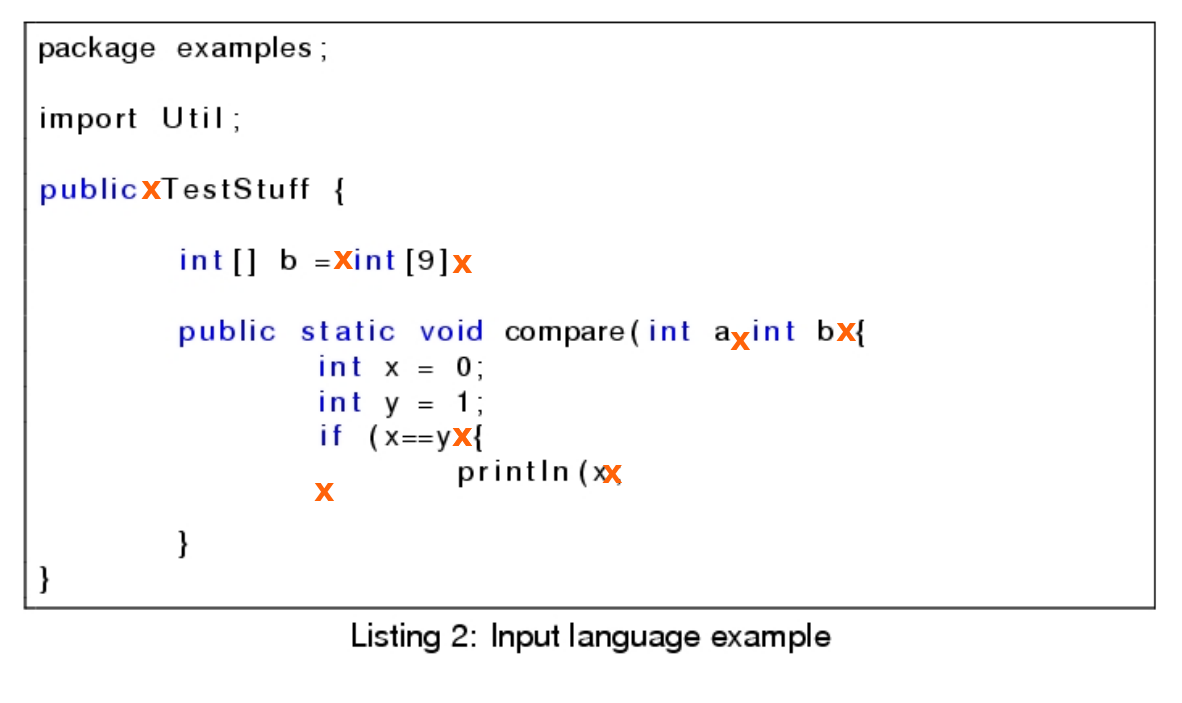
\includegraphics[width=12.5cm,height=8cm]{images/synError.png}
%\end{center}
\end{figure}

%,label={synErrors}]
%\begin{lstlisting}[caption={Input language example}]
%package examples;
%
%import Util;
%
%public TestStuff {
%
%	int[] b = int[9]
%	
%	public static void compare(int a int b {
%		int x = 0;
%		int y = 1;
%		if (x==y {
%			println(x;
%		
%	}
%}
%\end{lstlisting}
\newpage
The output of the console, after compiling the file in listing 2:
\begin{verbatim}
Warning: missing symbol: CLASS in line 5
Warning: missing symbol: NEW in line 7
Warning: missing symbol: SEMICOLON in line 9
Warning: missing symbol: COMMA in line 9
Warning: missing symbol: RPAREN in line 9
Warning: missing symbol: RPAREN in line 12
Warning: missing symbol: RPAREN in line 13
Warning: missing symbol: RBRACES in line 18
\end{verbatim}


\subsection {Type safety}
\label{labelTypeCheck}
We create a type description for every type we support, for primitive types (integer,boolean,character) as well as for extended types (modules).
A type descriptor is implemented as an object and holds following information: 

\begin{tabular}{lp{6cm}}
\texttt{int form} & Kind of the type, module,array,primitive \\
\texttt{int len} & This field is for arrays only, it contains the number of elements. \\
\texttt{DataType base} & For arrays only, it contains the type of the elements \\
\texttt{SymbolTableList fields} & The symboltable of an imported module is stored here. \\
\texttt{int size} & Size contains the size of a module. \\
\end{tabular}

For primitive types we have implemented types as final. For modules we create the type description dynamically. When we parse an import
statement we read the symbolfile of the appropriate module $x$ and create a type description for $x$.

\subsubsection{Type checking}
Type checking occurs in several code parts:

\paragraph{Naming convention}
We ensure that variable names are unique within it's scope. Local variables can have the same name as global variables or other local variables
of an another method. Every symbol (variable,method) has a unique name and a certain type. 

\paragraph{Operations on types}
Certain operations make only sense on designed types. We ensure that arithmetic and boolean operations work on appropriate authorized
types only. Arithmetic operators ${+,-,*,/}$ does only work with integer types. 
Relations ${>,<,>=,<=,==,!=}$ work on primitive data types only. On these operations we check if the type of the variable
 is the same before and after the operator.
Boolean operations ${\&\&,||}$ can treat expressions of different types. 

\paragraph{Assignments}
In assignments we compare the type of the variable before and the expression afterward as well. On invalid type assignments the compiler
prints a error message and the line number where it occurred.



\section{Symboltable}
\label{labelSymboltable}

The symboltable is used to beware various information about symbols during compile time.
The Parser produces for every field (global variables, methods) and local variables an entry in the symboltable.
We distinguish between different scopes. The global scope and local scopes. Every
method declaration has an entry in the global scope. The method's variables (local variables) are stored in a sublist of the corresponding
method (local scope).

The Symboltable is represented by the symboltable list (SymbolTableList.java) which consists of cells (SymbolTableCell.java).
A cell holds following information:
\newline
\newline
\begin{tabular}{lp{6cm}}
\texttt{String name} & Name of the entry (Variable name, Method name,\ldots) \\
\texttt{ClassType classType} & kind of the entry: variable, array, procedure \\
\texttt{TypeDesc type} & data type: int, boolean, char \\
\texttt{String value} & the value of the variable, when available \\
\texttt{SymbolTableList methodSymbols} & methods have a sub list with symbol table cells (local scope)\\
\texttt{int offset} & offset is negative \\
\texttt{int size} & in 4 bytes (word) \\
\texttt{int proc} & program counter of methods (for fixups) \\
\texttt{boolean globalScope} & scope information \\
\end{tabular}

Imported modules have their own symboltable which are stored in a separate container. For every imported module it's symbolfile 
will be read and a symboltable created.
 To load a symbol from a imported module the name of the file must be specified, e.g. \texttt{Util.print()}.






